\documentclass{article}
\usepackage[utf8]{inputenc}
\usepackage{algorithm}
\usepackage{algorithmicx}
\usepackage{algpseudocode}
\usepackage{amsmath}

\title{CS6033 Assign No.1}
\author{Minghe Yang }
\date{February 2021}

\usepackage{natbib}
\usepackage{graphicx}

\begin{document}
\renewcommand{\algorithmicrequire}{\textbf{Input:}} 
\renewcommand{\algorithmicensure}{\textbf{Output:}}
\maketitle

\section{Hash tables}

\maketitle{1.}
\\
Picking $k$ from $n$ keys that are in same slot: $\binom{n}{k}$
\\
Probability of $k$ keywords in same slot:$(1/n)^k$
\\
Probability of $(n-k)$ keywords in other slots:$(1-\frac{1}{n})^{n-k}$
\\
So $Q_k$ is equal to:$(\frac{1}{n})^k(1-\frac{1}{n})^{n-k}\binom{n}{k}$
\\\\
\maketitle{2.}
\\Let $X_i$ to express numbers contained in slot $i$, $A_i$ to express $k$ keywords in slot i,
from question 1 we can know that: $P\{A_i\}=Q_k$.
\\So $P_k=P_r\{\substack{\max\\i\leq i\leq n}X_i=k\}=P_r\{A_1\cup A_2\cup\dots\cup A_n\}
\\\leq P_r\{A_1\}+P_r\{A_2\}+P_r\{A_3\}+\dots+P_r\{A_n\}=nQ_k$ 
\\\\
\maketitle{3.}
\\$Q_k=(\frac{1}{n})^k(1-\frac{1}{n})^{n-k}\binom{n}{k}\leq 
(\frac{1}{n})^k(\frac{n!}{k!(n-k)!})^k=\frac{n(n-1)(n-2)\dots(n-k+1)}{n_kk!}
\\\frac{1}{k!}=\frac{1}{\sqrt{2\pi k}(\frac{k}{e})^k(1+\theta(\frac{1}{n}))}
\leq \frac{e^k}{k^k}$
\\\\
\maketitle{5.}
\\$E[M]=\sum_{i=1}^n iP_r\{M=i\}
=\sum_{i=1}^\frac{c\lg n}{\lg \lg n} iP_r\{M=i\}+\sum_{i=1+\frac{c\lg n}{\lg \lg n}}^n iP_r\{M=i\}
\\\leq \frac{c\lg n}{\lg \lg n}\sum_{i=1}^\frac{c\lg n}{\lg \lg n} P_r\{M=i\}+n*\sum_{i=1+\frac{c\lg n}{\lg \lg n}}^n P_r\{M=i\}
\\\leq P_r\{M\textgreater \frac{c\lg n}{\lg \lg n} \}*n + P_r\{M\textless \frac{c\lg n}{\lg \lg n}\}*\frac{c\lg n}{\lg \lg n}$
\\$E[M] = P_r\{M \leq \frac{c\lg n}{\lg \lg n}\}*\frac{c\lg n}{\lg \lg n}+n*\sum_{i=1+\frac{c\lg n}{\lg \lg n}}^n P_r\{M=i\},
\\=P_r\{M\leq \frac{c\lg n}{\lg \lg n}\}*\frac{c\lg n}{\lg \lg n} + n*\sum_{i=1+\frac{c\lg n}{\lg \lg n}}^n P_i \textless \frac{c\lg n}{\lg \lg n}+n*n*1/n^2
\\=O(\frac{\lg n}{\lg \lg n}) $

\section{Minimum Spanning Tree}
\maketitle {2.}
\begin{algorithm}
    \caption{minimum spanning tree solution}
    \begin{algorithmic}[1]
    \Require Minimum spanning tree $T$, decreased weight $j$ for nodes $(u,v)$
    \Ensure new Minimum spanning tree $T$
    \State Find weight $k$ for nodes $(u,v)$ in T
    % \State Search loop through DFS?
    \If {$k\geq j$}
    \State remove $k$ from $T$
    \State add $j$ to $T$
    \EndIf  
    \State \Return T
    \end{algorithmic}
\end{algorithm}

\section{Simple Algorithms}
\maketitle{2.a}
\begin{algorithm}
    \caption{mult function}
    \begin{algorithmic}[1]
    \Require $x,y$
    \Ensure $mult.(x,y)$
    \Function{$mult$}{$x,y$}
    \If {x=0 or y=0}
    \State mlt = 0
    \Else 
    \State \Return $x*(y\ mod\ 2) + mult.(2x, \lfloor y/2 \rfloor$)
    \EndIf 
    \EndFunction
    \end{algorithmic}
\end{algorithm}
\\
\maketitle{3.2.b}
\\Solution:
First of all, $f(1,1)=1*1+0=1$
We can know that $\vert trunc(y/2)\vert <\vert y\vert $,
\\from the inductive hypothesis, $mult(2x, trunc(y/2)) =2*x*trunc(y/2)$.
\\So the return value is:
$2*x*trunc(y/2)+x*(y\ mod\ 2)
\\=x*(2*trunc(y/2)+2*(y/2-trunc(y/2)))
\\=x*(2*y/2)
\\=x*y$


\section{Critical Thinking}
\maketitle{1.}
Non of them can solve the Knapsack problem perfectly.
\\Like a set $S=\{3,4,6,7,9\}$ and $n=10$, 
\\if you pick the smallest items first, you'll get $\{3,4\}$, $7$ in total;
\\if you choose the biggest items first, you'll get $\{9\}$ instead;
\\While the actual answer could be both $\{3,7\}$ and $\{4,6\}$.
\\\\
\maketitle{3.}
Imagine you have coins with value$\{30,10,7,8,1\}$ and you want a total value of $45$ with least coins.
From greedy algorithm you'll reach local optimum like $\{30,10,1,1,1,1,1\}$
Global optimum should be $\{30,10,8,7\}$.
\\\\
\maketitle{4.}
7 races are necessary.
\\
1st-5th:Divided them into 5*5 groups and race them in groups.
\\name them $a_1-a_5, b_1-b_5, c_1-c_5, d_1-d_5, e_1-e_5$.
\\6th race for $a_1, b_1, c_1, d_1, e_1$, name the fastest horse $a_1$, which is also the fastest among tha pack, $e_5$ is the slowest in this race.
\\7th race for $a_2, b_1, b_2, c_1, c_2$. The fastest two in this race will be 2nd and 3rd horse of the pack.
\\ The first three horses shoud be :$a_1$, 1st and 2nd horse in the 7th race.

\section{Recursive function}
\maketitle{1.}

$f(0,0) = 0$

$f(1,0) = 0$

$f(1,1) 
    = g(f(1,0),1)
    = g(0,1)
    = S(g(0,0))
    = S(0)
    = 1$

$f(2,1)
    = g(f(2,0),2)
    = g(0,2)
    = S(g(0,1)) 
    = S(1)
    = 2$
   
$f(2,2) 
    = g(f(2,1),2)
    = g(g(f(2,0),2),2)
    = g(2,2)
    = S(g(2,1))$
    
    $= S(S(g(2,0)))
    = S(S(2))
    = 4$

$f(2,3)
    = g(f(2,2),2)
    = g(g(f(2,1),2),2)
    = g(g(g(f(2,0),2),2),2)$
    
    $= g(g(g(f(2,0),2),2),2)
    = g(g(g(0,2),2),2)
    = g(g(S(S(g(0,0))),2),2)$
    
    $= g(g(2,2),2)
    = g(S(S(g(2,0))),2)
    = g(4,2)$
    
    $= S(S(g(4,0)))
    = S(S(4))
    = 6$
\\\\
\maketitle{2.}
$f(x,y) = x*y$,pseudocode should be like:
\begin{algorithm}
    \caption{function }
    \begin{algorithmic}[1]
    \Require $x,y$
    \Ensure $f(x,y)$
    \Function {$f$}{$x,y$}
    \State out = 0
    \While {y != 0}
    \State y = y-1
    \State out = f(x, y)
    \For {$x\in[1, x]$}
    \State out = out + x
    \EndFor 
    \EndWhile 
    \State \Return out
    \EndFunction
    \end{algorithmic}

\end{algorithm}

\maketitle{3.}
\\
$f(6,5)$
\\
$=g(f(6,4),6)
=g(g(f(6,3),6),6)
=g(g(g(f(6,2),6),6),6)
=g(g(g(g(g(f(6,1),6),6),6),6),6)
=g(g(g(g(g(f(6,0),6),6),6),6),6)$
\\
$=g(g(g(g(g(0,6),6),6),6),6)
=g(g(g(g(s(g(0,5)),6),6),6),6)
=g(g(g(g(s(s(g(0,4))),6),6),6),6)
=g(g(g(g(s(s(s(g(0,3)))),6),6),6),6)
=g(g(g(g(s(s(s(s(g(0,2))))),6),6),6),6)
=g(g(g(g(s(s(s(s(s(g(0,1)))))),6),6),6),6)
=g(g(g(g(s(s(s(s(s(s(g(0,0)))))),6),6),6),6)
=g(g(g(g(s(s(s(s(s(s(0))))),6),6),6),6)
=g(g(g(g(6,6),6),6),6)$
\\
$=g(g(g(s(s(s(s(s(s(g(6,0))))))),6),6),6)
=g(g(g(s(s(s(s(s(s(6)))))),6),6),6)
=g(g(g(12,6),6),6)
=g(g(18,6),6)
=g(24,6)$
\\
$=s(s(s(s(s(s(g(24,0)))))))
=30$

\begin{figure}[h!]
    \centering
    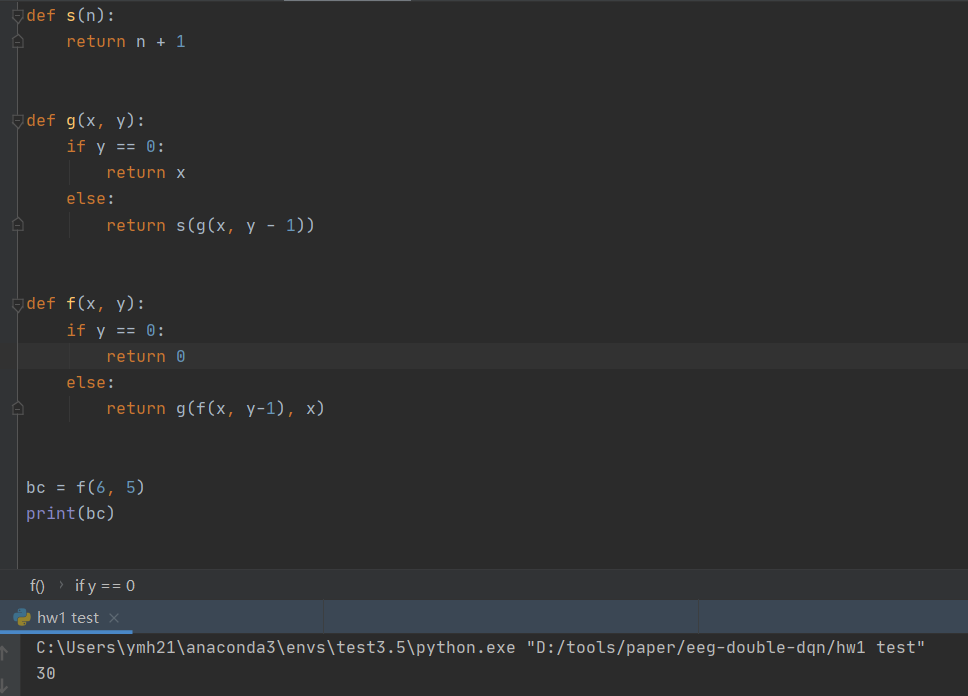
\includegraphics[scale=0.6]{hw10503.png}
    \caption{Python Verification}
    \label{fig:pv}
\end{figure}

\end{document}
